% !TeX spellcheck = nl_NL
\chapter{\IfLanguageName{dutch}{Stand van zaken}{State of the art}}
\label{ch:stand-van-zaken}

% Tip: Begin elk hoofdstuk met een paragraaf inleiding die beschrijft hoe
% dit hoofdstuk past binnen het geheel van de bachelorproef. Geef in het
% bijzonder aan wat de link is met het vorige en volgende hoofdstuk.

% Pas na deze inleidende paragraaf komt de eerste sectiehoofding.

Dit hoofdstuk gaat dieper in op de relevante inhoud van de GDPR voor dit onderzoek, en de mogelijke praktische oplossingen. 
Het einddoel is niet om een samenvatting te geven over de theoretische kant van de regelgeving, maar praktische oplossingen te bieden hoe bedrijven hun software 'GDPR-compliant' kunnen maken. 
Het is echter noodzakelijk enkele facetten toe te lichten zodat de lezer de nodige theoretische kennis heeft.
 Het dient als theoretische achtergrond om later (hoofdstuk 3) het effectieve onderzoek uit te voeren.
\section{{Hoofdelementen GDPR}}

\subsection{Juridisch}
De Europese commissie beschrijft de juridische aspecten van gegevensbescherming in \autocite{Eucom2018} als volgt.

\begin{itemize}
    \item \textbf{Grondrecht} Het Handvest van de grondrechten van de EU bepaalt dat EU-burgers recht hebben op bescherming van hun persoonsgegevens.
    \item \textbf{Wetgeving}: 
    \subitem \textbf{De algemene verordening gegevensbescherming} (GDPR): 
    Verordening (EU) 2016/679 betreffende de bescherming van natuurlijke personen in verband met de verwerking van persoonsgegevens en betreffende het vrije verkeer van die gegevens.
    \subitem \textbf{De politierichtlijn}: 
    Richtlijn (EU) 2016/680 betreffende de bescherming van natuurlijke personen in verband met de verwerking van persoonsgegevens door bevoegde autoriteiten met het oog op de voorkoming, het onderzoek, de opsporing en de vervolging van strafbare feiten of de tenuitvoerlegging van straffen, en betreffende het vrije verkeer van die gegevens.
   
\end{itemize}

In dit onderzoek wordt verder gebruik gemaakt van de richtlijnen uitgeschreven binnen de GDPR. 

Verder hebben de EU-landen nationale autoriteiten voor gegevensbescherming aangewezen die dienen toezicht te houden op de bescherming van persoonsgegevens. Voor België is dit: 

\textit{Commission de la protection de la vie privée \\  Rue de la Presse 35 1000 Bruxelles \\  Website: http://www.privacycommission.be/ \\ 
    Art 29 WP Vice-President: Willem DEBEUCKELAERE, President of the Belgian Privacycommission} 

\begin{figure}[h]
    
\includegraphics[width=\linewidth]{CPVP.jpg}
    \caption{Commission de la vie privée}
    http://www.anonymizedata.com/
\end{figure}


Tot slot is er nog een Europees Comité voor gegevensbescherming. In \textcite{Eucom2018} wordt gesteld dat het comité ruime bevoegdheden heeft om geschillen tussen de nationale toezichthoudende autoriteiten te beslechten, adviezen te geven en richtsnoeren vast te stellen over essentiële aspecten van de algemene verordening gegevensbescherming en de politierichtlijn.

\subsection{{Begrippen}}
http://www.privacy-regulation.eu/nl/artikel-4-definities-EU-AVG.htm
In artikel 4 van de GDPR worden definities gegeven van bepaalde termen die worden gebruikt. Hier volgt wat extra toelichting bij de belangrijkste termen. 

\subsubsection{Persoonsgegevens} 
Definitie: alle informatie over een geïdentificeerde of identificeerbare natuurlijke persoon ("de betrokkene"); als identificeerbaar wordt beschouwd een natuurlijke persoon die direct of indirect kan worden geïdentificeerd, met name aan de hand van een identificator zoals een naam, een identificatienummer, locatiegegevens, een online identificator of van een of meer elementen die kenmerkend zijn voor de fysieke, fysiologische, genetische, psychische, economische, culturele of sociale identiteit van die natuurlijke persoon.

 Als verder in dit onderzoek wordt gesproken over persoonlijke data, persoonsgegevens, persoonlijke gegevens, etc., gaat het over data die bovenstaande definitie volgt. 

Er zal vaak ter sprake komen dat de persoonsgegevens \textit{verwerkt} worden, de definitie hiervan luidt als volgt: een bewerking of een geheel van bewerkingen met betrekking tot persoonsgegevens of een geheel van persoonsgegevens, al dan niet uitgevoerd via geautomatiseerde procedés, zoals het verzamelen, vastleggen, ordenen, structureren, opslaan, bijwerken of wijzigen, opvragen, raadplegen, gebruiken, verstrekken door middel van doorzending, verspreiden of op andere wijze ter beschikking stellen, aligneren of combineren, afschermen, wissen of vernietigen van gegevens.

\subsubsection{Pseudonimisering} 
Het verwerken van persoonsgegevens op zodanige wijze dat de persoonsgegevens niet meer aan een specifieke betrokkene kunnen worden gekoppeld zonder dat er aanvullende gegevens worden gebruikt, mits deze aanvullende gegevens apart worden bewaard en technische en organisatorische maatregelen worden genomen om ervoor te zorgen dat de persoonsgegevens niet aan een geïdentificeerde of identificeerbare natuurlijke persoon worden gekoppeld. 

\subsubsection{Toestemming} 
De regelgeving is er in de eerste plaats gekomen om mensen te beschermen. Al te vaak werd in het verleden op een dubieuze manier toestemming gevraagd voor de verwerking van persoonsgegevens, en verstonden de betrokken gebruikers niet wat dat allemaal inhield. Daarom stelt de EU nu dat gebruikers heel duidelijk moeten weten welke data ze vrijgeven en wat er met die data mag/zal gedaan worden, en dit moet gepresenteerd worden in ondubbelizinnige, begrijpbare taal.
De toestemming moet specifiek zijn; er kan dus nooit meer een checkbox komen: “Hierbij stem ik in om al mijn persoonlijke info ter beschikking te stellen aan de organisatie”.\\ Definitie \textit{toestemming van de betrokkene}: elke vrije, specifieke, geïnformeerde en ondubbelzinnige wilsuiting waarmee de betrokkene door middel van een verklaring of een ondubbelzinnige actieve handeling hem betreffende verwerking van persoonsgegevens aanvaardt. 


\subsubsection{Inbreuken} 
Het moet ten alle koste vermeden worden, maar het is niet uitgesloten dat bepaalde persoonsgegevens ongewild worden verspreidt. Denk aan hackers, data-leaks etc. 
De definitie wordt alsvolgt gesteld: een inbreuk op de beveiliging die per ongeluk of op onrechtmatige wijze leidt tot de vernietiging, het verlies, de wijziging of de ongeoorloofde verstrekking van of de ongeoorloofde toegang tot doorgezonden, opgeslagen of anderszins verwerkte gegevens; 

\subsection{Rechtmatigheid van verwerking} www.privacy-regulation.eu
Als organisatie of rechtspersoon in het algemeen moet je er van uitgaan dat het verzamelen van persoonsgegevens standaard verboden is. Als je er toch gebruik van wilt maken, moet aan minstens één van de volgende voorwaarden voldaan worden. 
\begin{itemize}
    \item \textbf{Toestemming:} Gegevensverwerking kan enkel indien er de betrokkene expliciet toestemming (zie sectie 2.1.2) heeft gegeven om (beperkt) met zijn persoonlijke data aan de slag te gaan en die te verwerken. \\
    
    \item \textbf{Noodzaak}: De verwerking is noodzakelijk voor de uitvoering van een overeenkomst waarbij de betrokkene partij is, of om op verzoek van de betrokkene vóór de sluiting van de overeenkomst maatregelen te nemen. \\
    
    \item \textbf{Voldoen aan wettelijke verplichting }: de verwerking is noodzakelijk om te voldoen aan een wettelijke verplichting die op de verwerkingsverantwoordelijke rust; \\
    
     \item \textbf{Bescherming van vitale belangen}:  de verwerking is noodzakelijk om de vitale belangen van de betrokkene of van een andere natuurlijke persoon te beschermen. \\
    
    \item \textbf{Algemeen belang}: de verwerking is noodzakelijk voor de vervulling van een taak van algemeen belang of van een taak in het kader van de uitoefening van het openbaar gezag dat aan de verwerkingsverantwoordelijke is opgedragen. \\
    
     \item \textbf{Behartiging van de belangen}: de verwerking is noodzakelijk voor de behartiging van de gerechtvaardigde belangen van de verwerkingsverantwoordelijke of van een derde, behalve wanneer de belangen of de grondrechten en de fundamentele vrijheden van de betrokkene die tot bescherming van persoonsgegevens nopen, zwaarder wegen dan die belangen, met name wanneer de betrokkene een kind is. \\
\end{itemize}

\begin{figure}[h]
    \centering
    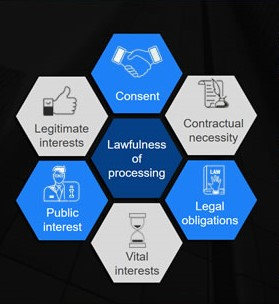
\includegraphics[scale=0.7]{six_pilars_processing.jpg}
    \caption{6 voorwaarden om rechtmatig gegevens te verwerken, schematische voorstelling.}
    https://www.i-scoop.eu/gdpr/legal-grounds-lawful-processing-personal-data/
\end{figure}


\section{{Onderwerpen geschikt voor technische implementaties}}

Er zijn heel wat stappen die een bedrijf kan ondernemen om op een veiligere manier om te gaan met hun gegevens en om te voldoen aan de richtlijnen die voorgeschreven worden. 
In de regelgeving wordt een verschil gemaakt tussen kleine/grote organisaties, of in grote mate persoonlijke gegevens verwerkt worden of niet, en dergelijke. In dit werk wordt gefocust op kmo's die een grote hoeveelheid persoonlijke gegevens verwerken, en hoe die specifiek de software die ze daarvoor gebruiken kunnen aanpassen. 


\subsection{Data security}
De meest voor de hand liggende. 

\subsection{Toestemming van de gebruiker}
In sectie 2.1.2 wordt toegelicht wat het volgens de GDPR begrepen wordt onder toestemming van de gebruiker. Het is één van de zes opties om te kunnen overgaan tot gegevensverwerking. De GDPR focust vooral op de begrijpelijkheid en duidelijkheid waar de gebruiker toestemming tot geeft. Er zijn vier “voorwaarden voor toestemming” opgenomen in de wetgeving. 
\begin{itemize}
    \item  Als je gegevens verwerkt op basis van toestemming, moet je als organisatie ten alle tijde bewijs kunnen leveren dat de betrokkene specifiek voor elke soort gegevens toestemming heeft gegeven. 
    \item  Het verzoek dient in een \textbf{begrijpelijke en gemakkelijk toegankelijke vorm en in duidelijke en eenvoudige taal} opgesteld te zijn. 
    \item  
    De toestemming kan ten alle tijde \textbf{ingetrokken worden}, en dit proces is even eenvoudig als het het geven ervan. 
\end{itemize}


 

\subsection{Pseudo- en anonimisatie van gegevens}
https://gdpr-info.eu/recitals/


De GDPR is van kracht op persoonsgegevens. Een manier om je data te kunnen gebruiken zonder aan de strenge regelgeving te moeten voldoen is door middel van je data te anonimiseren. Dit wil zeggen dat je verkregen data niet langer traceerbaar is tot de specifieke persoon van wie het afkomstig is. Volgens recital 26\footnote{Zie recital 26 in de bijlage.} valt geanonimiseerde data niet meer onder de GDPR. 

Voor veel bedrijven is volledig anonimiseren van data minder interessant. Een iets minder drastische oplossing is pseudonimisatie. Hierbij zorg je ervoor dat de uitgevoerde anonimisatie omkeerbaar blijft.  
Bij deze techniek ga je bepaalde velden, die heel duidelijk herleidbaar zijn tot een individu, zoals naam, adres, ... vervangen door een pseudoniem.
Hoewel er bij anonimisatie duidelijk wordt gezegd dat de data niet meer onder de gdpr valt, is dit bij psuedonimisatie niet het geval. Dit ligt bij psuedonimisatie iets anders. De regelgeving stelt dat het een maatregel is die het risico van ongewenst verspreiden van persoonlijke data aanzienelijk kan verkleinen, en daarnaast kan bijdragen tot data protection by design. Maar er wordt ook expliciet vermeld in Recital 28 dat pseudonimisatie de andere maatregelen niet uitsluit, en de data dus nog steeds onder de gdpr valt. 
Er wordt heel duidelijk gesteld in de regelgeving dat psuedonimisatie wordt aangeraden, het een deel kan zijn van data protection by design en by default, indien je de data zo snel mogelijk pseudonimiseert, maar 

https://gdpr-info.eu/recitals/
Recital 26
1The principles of data protection should apply to any information concerning an identified or identifiable natural person. 2Personal data which have undergone pseudonymisation, which could be attributed to a natural person by the use of additional information should be considered to be information on an identifiable natural person. 3To determine whether a natural person is identifiable, account should be taken of all the means reasonably likely to be used, such as singling out, either by the controller or by another person to identify the natural person directly or indirectly. 4To ascertain whether means are reasonably likely to be used to identify the natural person, account should be taken of all objective factors, such as the costs of and the amount of time required for identification, taking into consideration the available technology at the time of the processing and technological developments. 5The principles of data protection should therefore not apply to anonymous information, namely information which does not relate to an identified or identifiable natural person or to personal data rendered anonymous in such a manner that the data subject is not or no longer identifiable. 6This Regulation does not therefore concern the processing of such anonymous information, including for statistical or research purposes.

\begin{figure}[h]
    \includegraphics[width=\linewidth]{anonymise.jpg}
    \caption{Data anonymisation schematische voorstelling}
    http://www.anonymizedata.com/
\end{figure}


\subsection{Data access control.}
Een overweging die zeker kan gemaakt worden is welke documenten voor welke personen toegankelijk zijn. Laat ons het het voorbeeld nemen van een kmo die voor bepaalde projecten gegevens verzamelt. Dan moeten enkel de personeelsleden die aan dit project meewerken toegang hebben tot die gegevens.  Vaak zien we echter zo dat er een gemeenschappelijke locatie is waar alle gegevens worden bijgehouden, en die toegankelijk is voor alle werknemers. 

\subsection{Voldoen aan de rechten van de betrokkene}

Eén van de hoofdonderwerpen die de GDPR aansnijdt zijn de rechten van de betrokkene in verband met zijn gegevens. Zelfs al heeft die persoon oorspronkelijk toestemming gegeven om zijn gegevens te verzamelen en verwerken behoudt de volgende rechten.

\subsubsection{Verzoek tot verwijderen}
Het technische deel van dit onderzoek zal hier de focus op leggen. Met name wanneer een gebruiker het verzoek indient om al de gegevens die je als organisatie van die persoon bijhoudt, te verwijderen. De eerste stappen die je dan logischerwijs onderneemt is het anonimiseren van zijn opgeslagen gegevens. Denk aan adres, telefoonnummer, enzoverder. 

\subsubsection{Wat met Back-ups}

\subsubsection{Reacties op openbare fora}
Menig organisaties die onderzoek uitvoeren, maken gebruik van openbare fora. Denk aan reacties op een post op Facebook. Wanneer zo'n forum eigendom is van de organisatie, en zij beslissen welke content er online blijft en opgeslagen wordt, moet ook hier nagedacht worden over de GDPR. Stel, een gebruiker reageert op een post over Hiv-remmers het volgende: \textit{”Ik vind merk X niet goed, want ik woon in straat Y in dorp Z en ze komen hier niet leveren aan de deur, waardoor A(mijn zoon 12) er altijd om moet in het weekend.”}
Op basis van dit bericht is het niet moeilijk om te concluderen over wie het gaat, en kan een buitenstaander dus afleiden dat die persoon Hiv-positief is. Wat leidt tot de vraag: wat als deze persoon aan de organisatie vraagt om alle persoonlijke gegevens te verwijderen. Dan kan je nog al zijn gegevens in je database anonimiseren, als reacties als deze blijven bestaan heb je niet aan zijn verzoek voldaan. Dat brengt ons naadloos bij het volgende punt: Artificële intelligentie. 

\section{Artificiële intellegentie en GDPR.}
In het recente verleden heeft Artificiële Intelligentie en bij uitbreiding Machine Learning een geweldige evolutie gemaakt. AI, waarbij vele mensen nog veel te vaak denken aan robotjes die als mensen functioneren, staat ongetwijfeld in zijn kinderschoenen. Er zijn echter al zeer veel toepassingen, ontwikkeld door de 'grotere spelers' uit de informaticawereld, die al zeer goed werk leveren en voor iedere software developer beschikbaar zijn. Deze toepassingen bieden oplossingen voor het probleem dat PII zich in vele verschillende vormen kan aanbieden, en niet altijd door scripts wordt herkend.  Bijvoorbeeld: je wil ervoor zorgen dat foto's verwijderd worden waar persoonlijke info op staat, maar neutrale foto's behouden. Hier kan AI een oplossing bieden. 

\subsection{Aanbieders API's voor PII-herkenning}
Een KMO die wil gebruik maken van AI hoeft dus zelf helemaal geen eigen neurale netwerken op te stellen en moeilijke wiskunde berekingen uitvoeren. Een beter optie is om gebruik te maken van bestaande API's die achter de schermen deze artificiële intelligentie gaan uitvoeren. Hiervoor zijn de laatste jaren talloze opties ontwikkeld. In dit onderzoek zullen de twee grootste aanbieders besproken worden, namelijk \textit{Microsoft} met hun \textit{Azure Cognitive Services} en  \textit{Google Cloud Machine Learning} platform. In de volgende secties worden deze twee aanbieders met elkaar vergeleken op vlak van functionaliteit.
\begin{figure}[h]
    \centering
    \begin{subfigure}{0.5\textwidth}
        \centering
        
\includegraphics[width=.4\linewidth]{cognitive_services.png}
        \caption{Microsofts' Azure cognitive services}
        \label{fig:sub1}
    \end{subfigure}%
    \begin{subfigure}{0.5\textwidth}
        \centering
        \includegraphics[width=.4\linewidth]{google_cloud_ml.png}
        \caption{Google cloud machine learning.}
        \label{fig:sub2}
    \end{subfigure}
    \caption{De twee grootste aanbieders van een API voor machine learning solutions.}
    \label{fig:test}
\end{figure}

\subsection{Gezichtsherkenning}
De toepassing van machine-learning die ongetwijfeld het wijdst verspreid en verst geëvolueerd is. Dankzij zijn vele implementaties in smartphones, beveiligingsapparatuur, ... is gezichtsherkenning een zeer betrouwbare én snelle technologie geworden. Het is dan ook weinig verrassende dat beide aanbieders (Microsoft en Google) het ter beschikking stellen. 

Op vlak van gebruiksvriendelijkheid wint Microsoft zonder enige moeite. Na enkele minuten opzoekingswerk kom je al snel uit bij een demo hoe je 'Face detection in images' kan gebruiken. 


\begin{figure}[h]
    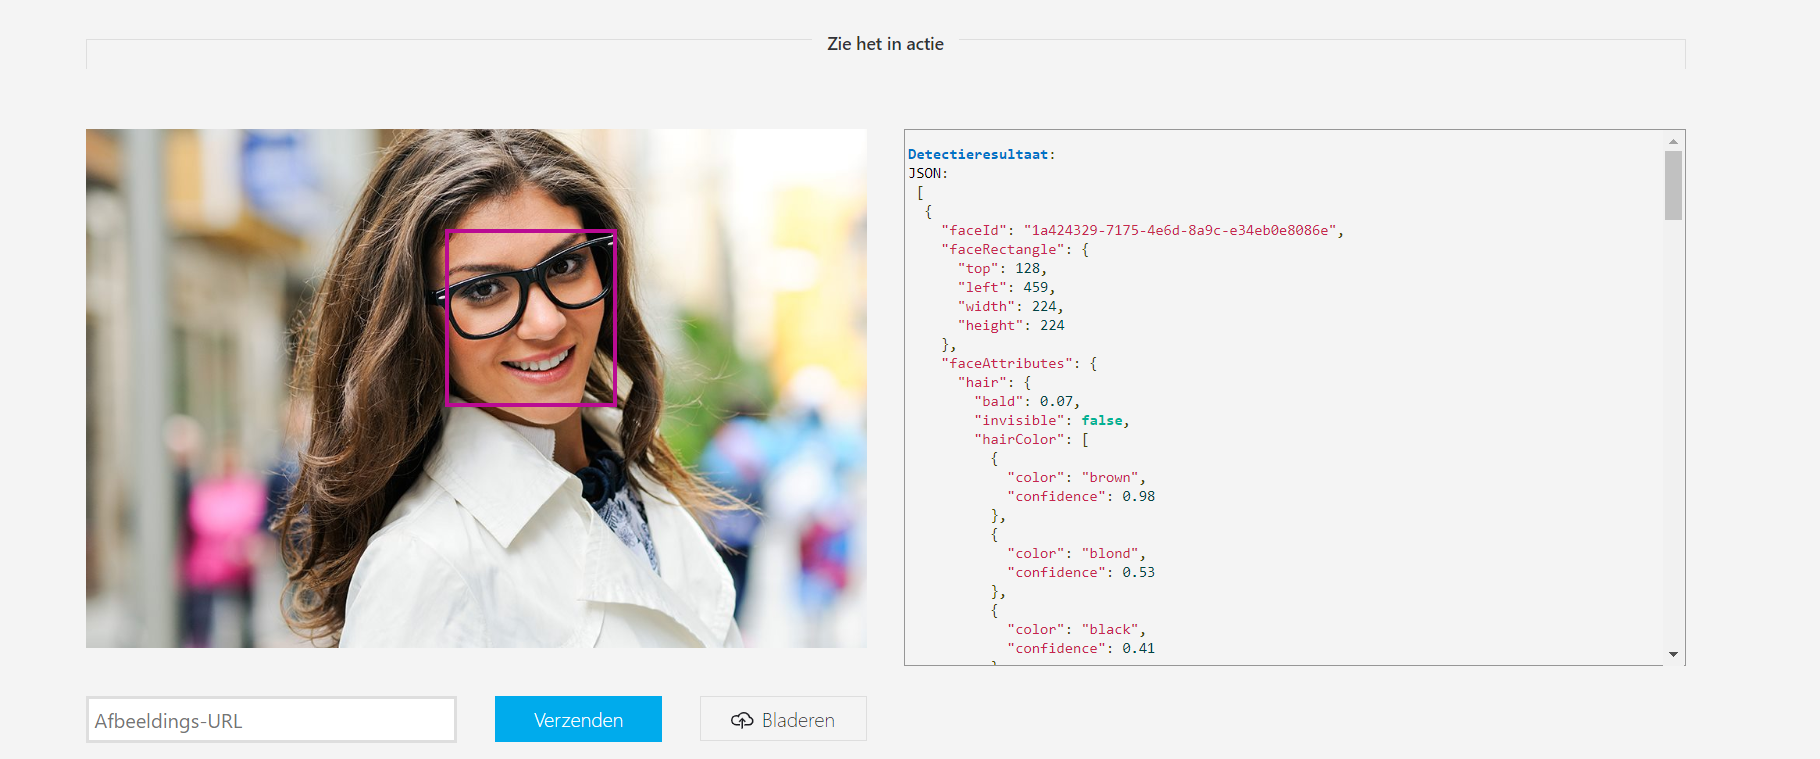
\includegraphics[width=\linewidth]{Face_recogn_micros_1.png}
    \caption{Cognitive services - Face recognition. Links de foto, rechts een JSON-file met herkende elementen.}
    \label{fig:cognitive}
\end{figure}

Op \hyperref[fig:cognitive]{figuur 2.5} zie je de gezichtsherkenning van Microsoft in werking. Links een foto met een duidelijk herkenbaar gezicht. Rechts zie je het resultaat. Er wordt een JSON-file uitgeprint met alle herkende elementen. Het eerstgevonden element is het face-id. Dit is de indicator die toont dat een gezicht herkend is. Daarna krijg je nog een heel wat extra elementen, die tot nog toe niet van belang zijn. 

Op de beschikbare demo zijn ook heel wat foto's beschikbaar met meerdere gezichten.

\begin{figure}[h]
    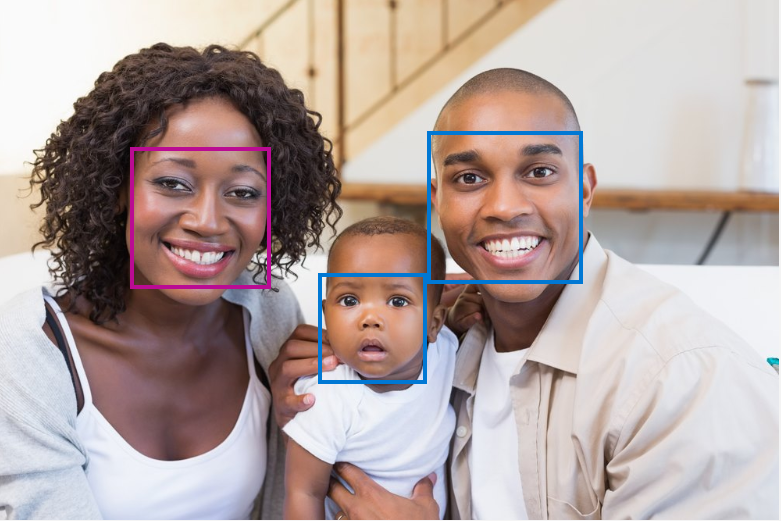
\includegraphics[width=\linewidth]{Face_recogn_micros_2.png}
    \caption{Cognitive services - Face recognition. Links de foto, rechts een JSON-file met herkende elementen.}
    \label{fig:cognitive}
\end{figure}

Je hebt dus heel wat info over de foto, en hier kan je in kader van persoonlijke informatie meer dan genoeg terug vinden. 


\section{{Uitleg Hogent}}
Dit hoofdstuk bevat je literatuurstudie. De inhoud gaat verder op de inleiding, maar zal het onderwerp van de bachelorproef *diepgaand* uitspitten. De bedoeling is dat de lezer na lezing van dit hoofdstuk helemaal op de hoogte is van de huidige stand van zaken (state-of-the-art) in het onderzoeksdomein. Iemand die niet vertrouwd is met het onderwerp, weet nu voldoende om de rest van het verhaal te kunnen volgen, zonder dat die er nog andere informatie moet over opzoeken \autocite{Pollefliet2011}.

Je verwijst bij elke bewering die je doet, vakterm die je introduceert, enz. naar je bronnen. In \LaTeX{} kan dat met het commando \texttt{$\backslash${textcite\{\}}} of \texttt{$\backslash${autocite\{\}}}. Als argument van het commando geef je de ``sleutel'' van een ``record'' in een bibliografische databank in het Bib\LaTeX{}-formaat (een tekstbestand). Als je expliciet naar de auteur verwijst in de zin, gebruik je \texttt{$\backslash${}textcite\{\}}.
Soms wil je de auteur niet expliciet vernoemen, dan gebruik je \texttt{$\backslash${}autocite\{\}}. In de volgende paragraaf een voorbeeld van elk.
\textcite{Lusignan2014} \textcite{ronnie}

\textcite{Knuth1998} schreef een van de standaardwerken over sorteer- en zoekalgoritmen. Experten zijn het erover eens dat cloud computing een interessante opportuniteit vormen, zowel voor gebruikers als voor dienstverleners op vlak van informatietechnologie~\autocite{Creeger2009}.

[7-20]
